\documentclass[12pt]{article}

\usepackage{sbc-template}

\usepackage{graphicx,url}

%\usepackage[brazil]{babel}   
\usepackage[utf8]{inputenc}  
     
\sloppy

\title{Banco de dados em tempo real: Firebase}

\author{Fábio da Silva Takaki\inst{1}, Lucas Martins Valladares Ribeiro\inst{1} }


\address{Faculdade de Ciências e Tecnologia\\
  Universidade Estadual Paulista \\
  "Júlio de Mesquita Filho" \\
  Caixa Postal 19060-900  -- Presidente Prudente -- SP -- Brasil
  \email{fabio@takaki.me, lucasmbtos@live.com}
}

\begin{document} 

\maketitle

\begin{abstract}
   With the emergence of the digital society and the Internet of Things, several concepts for data storage and manipulation have emerged with the purpose of reducing resource and maintenance costs of which Cloud Computing stands out. This article proposes a case study of a tool that addresses one of the service models of the Cloud Computing (IaaS, PaaS and SaaS) architecture, which is Firebase, a tool created by Google. Firebase is a mobile platform that provides a number of services for the rapid development of high-quality mobile applications, from which stand out the real-time database service that will be the focus of this work.
\end{abstract}
     
\begin{resumo} 
   Com o surgimento da sociedade digital e a Internet das Coisas, diversos conceitos para armazenamento e manipulação dos dados surgiram com a finalidade de diminiuir os custos de recursos e manutenção do qual destaca-se o Cloud Computing. Este artigo propõe um estudo de caso de uma ferramenta que aborda um dos modelos de serviço da arquitetura Cloud Computing (IaaS, PaaS e SaaS) que é o Firebase, uma ferramenta criada pela Google. O Firebase é uma plataforma mobile que fornece diversos serviços para o rápido desenvolvimento de aplicativos móveis de alta qualidade, do qual destaca-se o serviço de banco de dados em tempo real que será o foco principal deste trabalho.
\end{resumo}


\section{Introdução}

%  descrição do cenário e problemas em aberto
A popularização da internet gerou uma sociedade digital, o que antigamente era local, tornou-se online. O volume de informações se propagou de forma abundante nos últimos anos, principalmente com o avanço das tecnologias móveis. Em decorrência disso, diversos conceitos para armazenamento e manipulação dos dados surgiram com a finalidade de diminuir os custos de recursos e manutenção. Assim, surgiram diversos serviços para suprir a escalabilidade de recursos, como: \cite{WA} \cite{GAE} \cite{AWS}, que seguem conceitos de um modelo novo de armazenamento e manipulação de dados, o Cloud Computing. Até então, não existiam serviços que supriam as necessidades essenciais de serviços voltados para aplicativos atuais (chats e redes sociais), que demandam desenvolvimento móvel/web com armazenamento e sincronização de dados em tempo real. Este artigo apresenta um estudo de caso do Firebase, que tem por finalidade fornecer um serviço de dados em nuvem em tempo real, utilizado para criação de aplicativos multiplataformas que compartilham um banco de dados não relacional que a própria ferramenta disponibiliza, do qual será o foco principal deste trabalho. Como consequência, a ferramenta possibilita os desenvolvedores criarem aplicativos de alta qualidade de forma rápida e fácil, sem a necessidade de se preocupar com infraestrutura e escalabilidade de recursos.
\\
Este artigo está organizado da seguinte maneira: na Seção II será apresentado uma fundamentação teórica; na Seção III será apresentado a metodologia de desenvolvimento aqui aplicada; na Seção IV um estudo de caso da ferramenta firebase em que é realizado um estudo do desenvolvimento de uma aplicação; por fim na Seção V resultados e trabalhos futuros.

\section{Cloud Computing} \label{sec:firstpage}

Cloud computing é uma tecnologia em que os recursos de hardware e software, tais como aplicações especiais, CPU, armazenamento e muitos outros são fornecidos aos usuários através da Internet como um serviço, e é cobrado com base no que você usa \cite{1}. Como os recursos são fornecidos através da Internet, o usuário não se preocupa com a manutenção e suporte deles. Esses recursos têm a capacidade de escalabilidade automática de acordo com a demanda do cliente. 

O conceito de Cloud Computing é classificado em três modelos de serviço: Software as a Service (SaaS), Plataform as a Service (PaaS) e Infrastructure as a Service (IaaS). Com isso, é possível criar uma representação dos modelos de serviço por meio de camadas de virtualização (Figura~\ref{fig:architeture}).

\begin{figure}[ht]
\centering
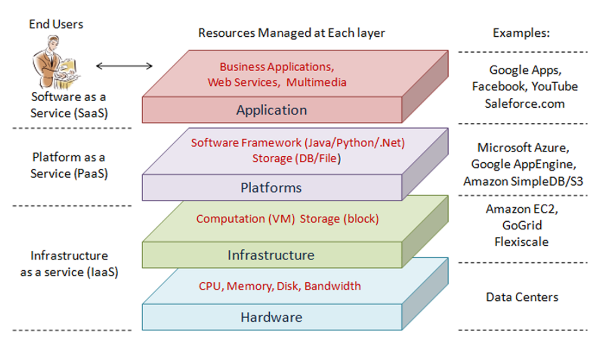
\includegraphics[width=.9\textwidth]{architeture.png}
\caption{Arquitetura Cloud Computing (retirado de: \cite{2})}
\label{fig:architeture}
\end{figure}

\textbf{Infrastructure as a Service}

O serviço oferece, como o próprio nome já diz, a infraestrutura. Compondo a base das camadas de virtualização, é responsável pelo hardware.
Ao invés de manter hacks, servidores e roteadores, o usuário contrata sevidores virtuais, que armazenarão de forma comum á aqueles. Os tipos de cobrança mais comuns são: número de servidores e o tráfego de dados utilizado.

\textbf{Platform as a Service}

Plataforma como serviço, tradução literal, é o serviço entre Infrastructure as a Service e Software as a Service. É proporcionar um ambiente ou plataforma apropriada na qual o desenvolvedor pode criar as aplicações e o software através da Internet sem necessidade de instalação ou gerenciar o ambiente de desenvolvimento \cite{1}. O serviço trás ao usuário um ambiente flexível e adequado que suporta as tecnologias que deseja, como frameworks ou linguagens de programação. Como observado na figura~\ref{fig:architeture}, temos o modelo de serviço Google App Engine, o qual oferece uma plataforma de desenvolvimento para aplicações web e móvel.

\textbf{Software as a Service}

Entrando na última camada de serviços, observamos o Software as a Service. Esse modelo propõe um software como serviço fornecido através da internet, não necessitando de sua instalação. O fornecedor deste modelo de serviço, é responsável por controlar e limitar o uso das aplicações. Portanto, o cliente deste modelo de serviço também fica livre da necessidade de uma infraestrutura, já disponibilizada pelo fornecedor.

Assim, com os conceitos de Cloud Computing, o Firebase é considerado Platform as a Service, por ser uma plataforma de desenvolvimento que oferece armazenamento e sincronização de dados em tempo real, utilizando apenas código client-side. 

\section{Metodologia de Apoio ao Firebase}  \label{sec:metodologia}

Firebase foi criado em 2011 por Andrew Lee and James Tamplin porém foi lançado oficialmente em 2012. Originalmente o sistema tinha o intuito de fornecer um banco de dados em tempo real fornecendo uma API aos usuários para armazenar e sincronizar dados através de diferentes clientes \cite{3}. Assim, a metodologia do Firebase mudou um pouco após a aquisição da Google. Dois anos depois de sua release, surgiu diversos serviços que complementam a ideia do banco de dados em tempo real, voltados para aplicativos móveis ou web: Firebase Auth, Firebase Storage, Firebase Cloud Messaging, Firebase Remote Config, Firebase Test Lab for Android e Firebase Crash Reporting. Dentre todos os serviços citados nesta seção, este trabalho foca no objetivo inicial do Firebase que é o real-time database.

\textbf{Firebase Realtime Database}

O Firebase Realtime Database é um banco de dados hospedado em nuvem. Os dados são armazenados como JSON e sincronizados em tempo real para cada cliente conectado. Ao criar aplicativos multiplataforma com nossos SDKs para iOS, Android e JavaScript, todos os seus clientes compartilham uma instância do Realtime Database e recebem automaticamente atualizações com os dados mais recentes \cite{Firebase}. Portanto, o objetivo do Firebase Realtime Database é fornecer um banco de dados em tempo real, em que o cliente é conectado diretamente e só  é preciso enviar os dados através de uma API.

\textbf{Como os dados são armazenados}

Todos os dados são armazenados na nuvem do Firebase em objetos JSON formando uma árvore. Quando um dado é adicionado no banco de dados, o dado se torna em um nó na árvore JSON do qual o Firebase associa uma chave à esse nó para manipulações futuras. Nesse sentido, um exemplo de um chat em que o usuário tem seu próprio perfil com sua lista de contatos, a árvore JSON se tornaria algo como na Figura~\ref{fig:json-tree}.

\begin{figure}[ht]
\centering
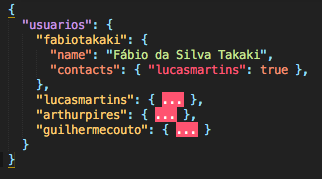
\includegraphics[width=.5\textwidth]{json-tree.png}
\caption{Exemplo de uma estrutura JSON de uma aplicação chat.}
\label{fig:json-tree}
\end{figure}


\textbf{Segurança e Regras}

O Firebase Realtime database tem uma área (Firebase Realtime Database Rules) onde há configurações e regras que determinam quem tem acesso a leitura e gravação no banco de dados, como os dados estão estruturados e o qual índices existem. Todas as regras ficam armazenadas nessa área do Firebase e podem ser alteradas a qualquer momento na ferramenta. Portanto, todas as operações de leitura e gravação só serão concluídas se as regras armazenadas no Firebase Realtime Database Rules permitirem. 

A estrutura em que as regras são definidas também são armazenadas em JSON que seguem uma syntax e são definidas em quatro tipos: 
\begin{enumerate}
  \item \textbf{.read} - Descreve se e quando os dados podem ser lidos pelos usuários.
  \item \textbf{.write} - Descreve se e quando os dados podem ser escritos.
  \item \textbf{.validate} - Define o aspecto correto de um valor formatado, se ele tem atributos filho e o tipo de dados.
  \item \textbf{.indexOn} - Especifica uma criança a indexar para suportar pedidos e consultas.
\end{enumerate}

O Firebase Realtime Database é pré-configurado com o Firebase Auth, que é responsável por realizar a segurança do app quando sua natureza são dados restritos aos usuários autenticados. Como o intuito deste trabalho é realizar um estudo de caso do serviço de banco de dados em tempo real, não será utilizado para o estudo de caso o Firebase Auth. Portanto, nossa estrutura JSON de permissões trataremos como aberta para a realização do estudo de caso sem a necessidade do Firebase Auth.



\section{Estudo de Caso}

Nesta seção é realizado um estudo de caso com os conceitos da ferramenta até então apresentada, no qual é analisado as funcionalidades e facilidades com a ferramenta Firebase real time database para a criação de um chat público em tempo real.

\textbf{Acesso e criação de projetos}

O acesso à todos os serviços (citados na Seção \ref{sec:metodologia}) do Firebase, é preciso apenas de uma conta Google, que pode ser criada gratuitamente. Concedido o acesso ao console do Firebase, facilmente você cria um projeto apenas especificando o nome do projeto, e assim é liberado o acesso à todos os serviços do Firebase, necessitando apenas do desenvolvedor configurar a aplicação web ou mobile desejada com as keys da API do Firebase.

\section{Conclusões e Trabalhos Futuros}

% as vantages do firebase e que a pesquisa pode ser expandida com os serviços de autenticação, storage
jsxjiosjoijsocj

\begin{table}[ht]
\centering
\caption{Variables to be considered on the evaluation of interaction
  techniques}
\label{tab:exTable1}
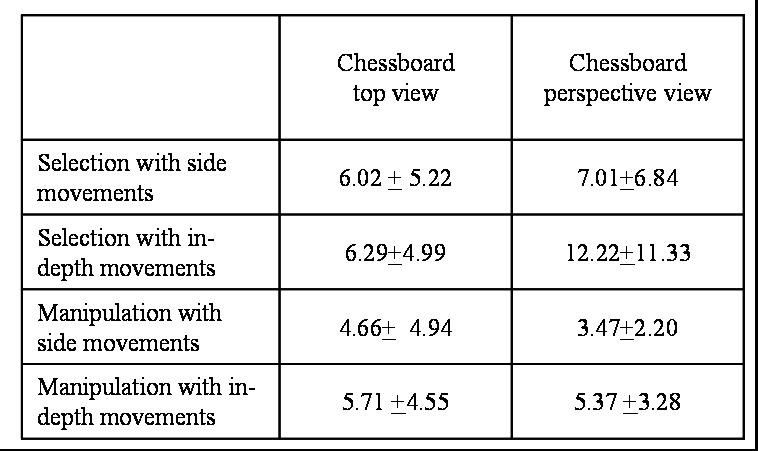
\includegraphics[width=.7\textwidth]{table.jpg}
\end{table}

\bibliographystyle{sbc}
\bibliography{bibliografia}

\end{document}
